\documentclass[letterpaper, twoside, 12pt,memoire]{thETS}
\usepackage{amsmath}
\usepackage{amsfonts}
\usepackage{amssymb}
\usepackage[utf8]{inputenc}
\usepackage{graphicx}
\usepackage{color}
\usepackage[T1]{fontenc}
\usepackage{subfigure}
\usepackage{float}
\usepackage[round]{natbibETS}
\usepackage{varwidth}
\usepackage{todonotes}

\newcommand{\LT}[1]{%
	{
	\todo[inline,color={red!33!green!33!blue!33}]{%
	\textbf{[LT]:}~#1}
	}}
	
\newcommand{\SC}[1]{%
	{
	\todo[inline,color={red!100!green!33!}]{%
	\textbf{[SC]:}~#1}
	}}

\newcommand{\fig}[1]{figure~\ref{#1}}

\begin{document}
\begin{chapter}{La norme H.264}
\LT{Traduire les images en francais (plus tard)}
La norme de compression vidéo H.264, aussi connue sous le nom
de MPEG-4 AVC, suscite un grand intérêt autant commercial que théorique, vu ses
gains en compression et les technologies de pointe qui la composent. Cette
norme, approuvée en mai 2003, raffine les technologies de ses prédécesseurs
MPEG-2 et H.263. De plus, elle intègre plusieurs innovations avant-gardistes. En
2011, H.264 est une norme incontournable pour les applications vidéos telles le
Blu-Ray, la télévision sur IP et la lecture vidéo en transit
(\textit{streaming}). Dans ce chapitre, nous présentons sommairement H.264 ainsi
que les rudiments de l'encodage vidéo.

\begin{section}{Les notions élémentaires de la vidéo numérique}
Avant de présenter les notions de blocs et de macroblocs, définissons une image
numérique comme un ensemble fini d'éléments d'image, nommés pixels, contraction
de la locution anglaise \textit{picture element}. Un pixel est une unité de
surface indivisible qui permet d'afficher une couleur (comme illustré à la
\fig{fig-PixelLighthouse}). La variation de l'intensité des composantes d'un
pixel permet d'afficher l'ensemble de couleurs contenues dans un espace
colorimétrique. Le choix de ce dernier détermine les composantes, leur nombre et
la portée de leur valeur. Un espace colorimétrique est un modèle mathématique
permettant l'expression numérique d'un ensemble de couleurs.

\begin{figure}[htb]
\centering
\fbox{
\includegraphics[width=0.25\linewidth]{images/PixelLighthouse.png}
}
\caption{Visualisation des pixels à l'intérieur d'une image numérique de la
suite d'images \textit{True Color Image Suite} de Kodak.}
\label{fig-PixelLighthouse}
\end{figure}

L'espace colorimétrique RVB est très populaire, son nom est l'acronyme des trois
couleurs qui le composent~: rouge, vert et bleu. Cependant, les composantes de
cet espace colorimétrique sont fortement corrélées avec la luminance
(intensité lumineuse); une augmentation de celle-ci occasionnera une
augmentation des valeurs des composantes RVB.

L'espace colorimétrique utilisé par la norme H.264 se nomme
YC$_{\text{B}}$C$_{\text{R}}$, Y représente la luminance, et C$_{\text{B}}$ et
C$_{\text{R}}$ sont, respectivement, les différentiels de Y par rapport au bleu
et au rouge, comme illustré à la figure~\ref{fig-YCBCR}. Les composantes
C$_{\text{B}}$ et C$_{\text{R}}$ sont aussi connues sous le nom de composantes
chromatiques, c'est-à-dire, relatives aux couleurs. La séparation de la
luminance et des composantes chromatiques réduit la corrélation entre les
composantes de cet espace colorimétrique.

\begin{figure}[htb]
\fbox{\begin{varwidth}{\textwidth}\centering
\subfigure[Lena]{
\includegraphics[width=0.22\linewidth]{images/lena.png}
}
\subfigure[Composante Y]{
\includegraphics[width=0.22\linewidth]{images/yLena.png}
}
\subfigure[Composante C$_{\text{B}}$]{
\includegraphics[width=0.22\linewidth]{images/cbLena.png}
}
\subfigure[Composante C$_{\text{R}}$]{
\includegraphics[width=0.22\linewidth]{images/crLena.png}
}
\end{varwidth}}
\caption{Composantes de l'espace colorimétrique YC$_{\text{B}}$C$_{\text{R}}$
pour l'image Lenna.}
\label{fig-YCBCR}
\end{figure}

Notons deux faits intéressants, que nous pouvons observer grâce à la
\fig{fig-YCBCR}. Premièrement, dans une image naturelle, il y a souvent beaucoup
moins de variation dans les composantes chromatiques que dans la composante Y.
Deuxièmement, le système visuel humain est beaucoup plus sensible aux variations
de luminance qu'à celles de C$_{\text{B}}$ et C$_{\text{R}}$ \citep{Wang2001}.
Ces deux constats sont à la base du sous-échantillonnage chromatique. Cette
approche vise à conserver plus d'échantillons Y que d'échantillons chromatiques.
La norme H.264 définit plusieurs ratios de sous-échantillonnage chromatique
permettant le contrôle du compromis entre la qualité visuelle et le nombre
d'échantillons chromatiques à encoder.

Les pixels d'une image naturelle témoignent d'une forte corrélation spatiale.
Basées sur cette propriété, certaines opérations d'encodage sont effectuées sur
des ensembles quadrilatéraux de pixels, nommés blocs. Dans un encodage par
blocs, l'image est séparée en blocs non chevauchants. La taille des blocs varie
selon la norme, mais sont généralement des multiples de quatre. Par exemple,
H.264 définit les tailles de blocs suivantes: $16 \times 16$, $8 \times 8$, $16
\times 8$, $8 \times 16$, $4 \times 4$, $8 \times 4$ et $4 \times 8$. Un bloc de
grande taille porte le nom de macrobloc. Dans la norme H.264, un macrobloc est
défini comme un bloc de taille $16 \times 16$.

Avant d'être séparée en macroblocs, une image est séparée en une ou plusieurs
tranches. Une tranche est un regroupement d'un ou plusieurs macroblocs. Les
macroblocs qui composent une tranche ne sont pas nécessairement contigus. La
particularité d'une tranche est qu'elle est encodée indépendamment des autres
tranches de l'image. Quoique cette approche réduise l'efficacité de l'encodage,
elle est particulièrement appréciée dans des contextes de parallélisme et de
résilience aux erreurs.
\end{section}

\begin{section}{Survol de la norme H.264}
La norme H.264 offre, pour une fidélité visuelle comparable à MPEG-2, une
économie de 50~\% du débit~\citep{sullivan2005}. Cette réalisation n'est
pas l'œuvre d'une seule innovation, mais bien de l'effet combiné de plusieurs
innovations importantes dans divers aspects de l'encodage vidéo. Pour mieux
comprendre cette technologie, décrivons d'abord sommairement les étapes
d'encodage vidéo. Par la suite, chaque étape sera expliquée dans les
sections subséquentes.

\begin{figure}[htb]
\centering
\includegraphics[width=0.75\linewidth]{images/encoderOverview.png}
\caption{Survol des étapes de la norme H.264~\citep{schafer2003}.}
\label{fig-EncoderOverview}
\end{figure}
\LT{Modifier les blocs de la \fig{fig-EncoderOverview} pour mieux s'arrimer avec
le texte.}

Comme illustré à la figure~\ref{fig-EncoderOverview}, le signal vidéo est divisé
en macroblocs. L'efficacité de la prédiction de macroblocs repose sur la forte
corrélation spatiotemporelle des pixels qui les composent. Dans un encodage
prédictif, ce ne sont pas les pixels du bloc qui sont encodés, mais bien le
différentiel entre le bloc et sa prédiction. Le différentiel, moins corrélé,
augmente l'efficacité de la compression~\citep{Drew2004}. Néanmoins, le coût lié
à l'utilisation du différentiel est l'encodage des données de prédiction. La
norme H.264 permet deux types de prédictions~: la première, basée sur les blocs
d'une autre trame (\textit{inter}) et la seconde, obtenue par l'interpolation du
contenu des blocs voisins d'une même trame (prédiction \textit{intra}). La norme prévoit aussi
une transformée entière ainsi qu'une quantification, toutes deux appliquées au
différentiel de la prédiction. Ces opérations augmentent l'efficacité de l'encodage
entropique d'où résulte un meilleur taux de compression. La transformée entière
ne fait que réorganiser les valeurs d'un bloc. La quantification est plus
importante. Elle est cruciale et permet le contrôle du compromis entre le nombre
de bits dédiés à l'encodage d'une trame (débit) et la qualité visuelle.
Finalement, la division du signal vidéo en macroblocs crée des effets de bloc
dans l'image, qui sont mitigés à l'aide d'un filtre antiblocs
(\textit{deblocking filter}).
\end{section}

\begin{section}{La prédiction de macroblocs}
\begin{subsection}{La prédiction de macroblocs \textit{inter}}
\newcommand{\ltMIN}[1]{\arg \min_{#1}}
\newcommand{\ltSAD}[1]{\textrm{SAD}(#1)}
\newcommand{\ltC}[1]{\mathbf{C}_{#1}}
\newcommand{\ltR}[1]{\mathbf{R}_{#1}}
Une source importante de redondance exploitée par la norme H.264 est la
redondance inter-image, souvent appelée \textit{inter}. La prédiction
\textit{inter} crée un modèle de prédiction basé sur une ou plusieurs trames
vidéo préalablement décodées~\citep{richardson2003}. Ce modèle de prédiction est
fondé sur la recherche et la compensation de mouvement dans le but d'accomplir
l'appariement de blocs entre deux trames.

\begin{figure}[htb]
\centering
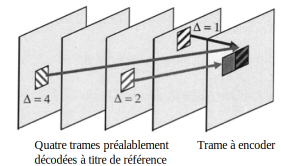
\includegraphics[scale=0.5]{images/multipicture.png}
\caption{Vecteurs de mouvement provenant de quatre trames vidéo préalablement
décodées, utilisées pour encoder les blocs dans la trame
courante~\citep{schafer2003}.}
\label{fig-MultiPicture}
\end{figure}

Un macrobloc contient $16 \times 16$ valeurs de luminances qui peuvent être
décomposées de quatre manières distinctes~: une partition $16 \times 16$, deux
partitions $16 \times 8$, deux partitions $8 \times 16$ et quatre partitions $8
\times 8$. De plus, chacun des sous-macroblocs $8 \times 8$ peut également être
décomposé~: deux partitions $8 \times 4$, deux partitions $4 \times 8$, et
quatre partitions  $4 \times 4$. Le tout est résumé à la
figure~\ref{fig-MacroblockPartitions}.

\begin{figure}[htb]
\centering
\includegraphics[scale=0.5]{images/MacroblockPartitions.png}
\caption{Partitions de macroblocs et de sous macroblocs~\citep{schafer2003}.}
\label{fig-MacroblockPartitions}
\end{figure}

La décomposition de macroblocs permet d'optimiser l'encodage selon le niveau de
détails d'une surface. Un macrobloc $16 \times 16$ est efficace pour les régions
lisses où le différentiel de la prédiction possède peu d'énergie, ou pour de
grandes zones où le mouvement est uniforme et translationnel. Des partitions
plus petites sont utiles pour des régions plus complexes où le différentiel
entre la prédiction et le macrobloc à encoder est élevé. La décomposition en
partitions permet d'utiliser plusieurs vecteurs de mouvements (un par partition)
pour mieux modéliser la surface. Cependant, les vecteurs de mouvements
supplémentaires doivent, eux aussi, être encodés, ce qui décourage l'usage
inutile de petites partitions.

Lorsque le nombre de partitions est élevé, encoder les vecteurs de mouvements de
chacune d'elles peut engendrer un coût binaire considérable et particulièrement
à bas débit. C'est pourquoi, dans la norme H.264, les vecteurs de mouvements
sont encodés différentiellement à l'aide de la médiane ou d'une prédiction
directionnelle guidée par les blocs voisins~\citep{wiegand2003}. Cette
prédiction est efficace, car la redondance spatiotemporelle cause une forte
corrélation entre les vecteurs de mouvements de blocs avoisinants. Les blocs
utilisés pour la prédiction sont des blocs préalablement décodés, qui
appartiennent à la même tranche que le bloc à prédire.

On peut remarquer, à la \fig{fig-EncoderOverview}, que la trame de référence
n'est pas utilisée pour la recherche de mouvement, mais bien la trame décodée.
Suite à l'encodage d'une trame, l'encodeur procède au décodage, afin d'obtenir
une trame identique à celle que possèderait un décodeur. Cette approche améliore
la précision des prédictions, car elle tient compte des artefacts dus à
l'encodage. Ceci explique pourquoi la recherche de vecteurs de mouvements est
effectuée dans les trames préalablement décodées.

Soit $(u,v)$ le vecteur de mouvement, issu de la recherche de mouvement à
l'intérieur d'une surface $[-p, p] \times [-p, p]$, entre le bloc à encoder et
le bloc le plus fidèle obtenu avec
\begin{equation}
\label{eq-Vectors}
(u, v) = \ltMIN{(u,v) \in [-p, p] \times [-p, p]} \ltSAD{u, v, \ltC{}, \ltR{}}
\:,
\end{equation}
où la somme de la différence absolue (SAD) d'un bloc de taille $M\times N$ à la position $(x,y)$
dans la trame courante $\ltC{}$, par rapport à une trame de référence $\ltR{}$,
se définit comme étant
\begin{equation}
\ltSAD{u,v, \ltC{}, \ltR{}} = \sum_{k=0}^{M-1}\sum_{l=0}^{N-1} \left|
\ltC{x+k,y+l} - \ltR{x+k+u,y+l+v} \right|\:.
\end{equation}

En supposant que le bloc à encoder et le bloc résultant de la recherche de
vecteurs de mouvements soient identiques, il ne suffirait que d'encoder
$(u,v)$ et le numéro de la trame de référence ($\Delta$, voir
figure~\ref{fig-MultiPicture}) pour représenter le bloc à encoder. Cependant, il
en est rarement ainsi; il est souvent nécessaire d'encoder le différentiel entre
le bloc prédit et le bloc à encoder.

De plus, $(u,v)$ n'est pas nécessairement composé d'entiers (le déplacement des
objets ne se fait généralement pas par des pas de pixels entiers). La norme
H.264 permet l'utilisation de vecteurs de mouvements offrant un dégré de
précision au quart de pixel. Deux approches d'interpolation distinctes sont
utilisées pour le demi et le quart de pixel. Le demi-pixel $\mathbf{b}$, dans la
figure~\ref{fig-HalfPel}, est obtenu à l'aide de l'équation suivante provenant
de l'application d'un filtre à réponse impulsionnelle finie~:
\begin{equation}
\mathbf{b} = \text{round} \left(\frac{E - 5F + 20G + 20H - 5I + J}{32}
\right)\:.
\label{eq-DemiPixel}
\end{equation}
Dans l'équation précédente, round arrondit à l'entier le plus proche. De
plus, E, F, G, H, I et J sont des positions des pixels illustrées à la
figure~\ref{fig-HalfPel}. 

\begin{figure}[htb]
\centering
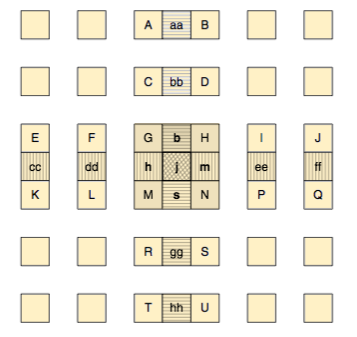
\includegraphics[scale=0.5]{images/HalfPel.png}
\caption{Interpolation au demi-pixel. Inspiré de~\cite{richardson2003}.}
\label{fig-HalfPel}
\end{figure}

À la figure~\ref{fig-HalfPel}, les lettres majuscules représentent des valeurs
de pixel en position entière; les minuscules sont des valeurs au demi-pixel,
sauf j qui est au quart de pixel. Pour les valeurs au quart de pixel,
l'interpolation linéaire de valeurs au demi-pixel est utilisée. Soit $\mathbf{a}$ une valeur au quart de
pixel située entre G et $\mathbf{b}$ dans la \fig{fig-HalfPel}. On obtient
$\mathbf{a}$ en effectuant
\begin{equation}
\mathbf{a} = \text{round} \left(\frac{G + \mathbf{b} }{2} \right)\:.
\end{equation}
Le filtre à réponse impulsionnelle finie de l'équation~\ref{eq-DemiPixel} ainsi
que l'interpolation linéaire précédente sont utilisés seulement pour la
luminance. Les composantes chromatiques sont obtenues à l'aide d'une
interpolation bilinéaire, comme illustré à la figure~\ref{fig-ChromaPel}

\begin{figure}[htb]
\centering
\includegraphics[width=0.5\linewidth]{images/ChromaPel.png}
\caption{Interpolation de la composante chromatique au huitième de pixel.
Inspiré de~\cite{richardson2003}.}
\label{fig-ChromaPel}
\end{figure}

Pour obtenir la composante chromatique de $\mathbf{a}$, on a recourt à
{\small\begin{equation}
\mathbf{a} = \text{round} \left( \frac{(8 - d_x) \cdot (8-d_y)A + d_x \cdot (8 -
d_y)B + (8 - d_x) \cdot d_yC + d_x \cdot d_yD}{64} \right)\:.
\end{equation}}
Où A, B, C, D sont les valeurs chromatiques des pixels entiers à une distance
$(d_x,d_y)$ entourant la valeur à interpoler.
\end{subsection}

\begin{subsection}{La prédiction de macroblocs \textit{intra}}
Une seconde source considérable de redondance exploitée par la norme H.264 est
la redondance spatiale à l'intérieur d'une image. La prédiction \textit{intra}
exploite cette redondance pour modéliser la texture d'un bloc à partir celle des
blocs avoisinants.

Comme c'est le cas pour la prédiction \textit{inter}, la prédiction
\textit{intra} repose sur le concept de blocs et de macroblocs et comprend la
notion de blocs à tailles variables visant à améliorer la prédiction de régions
complexes. La norme H.264 permet à l'encodeur de choisir entre des macroblocs
$16 \times 16$ ou des sous-blocs $4 \times 4$ pour la luminance. Selon le choix,
différents modes de prédiction sont offerts.

Deux faits intéressants sont à noter. Premièrement, la prédiction \textit{intra}
est accomplie dans le domaine spatial (contrairement à H.263 et MPEG-4 Visual
qui utilisent le domaine fréquentiel \citep{wiegand2003}). Deuxièment, le
recours aux pixels de blocs voisins pour établir une prédiction peut mener à une
propagation d'erreurs, si celle-ci repose sur des pixels corrompus.

Une prédiction intra précise engendre un différentiel faible et
décorélé, ce qui améliore le taux de compression issu des étapes subséquentes
de l'encodage. Les gains obtenus par l'usage de la prédiction justifient le coût
supplémentaire de l'encodage des données de la prédiction.


La norme H.264 définit neuf modes de prédiction liés à l'utilisation de blocs
$ 4 \times 4$, illustrés à la \fig{fig-4x4PredictionModes}. Huit de ces modes
sont des extrapolations directionnelles à des angles de 26.6$^\circ$, 45$^\circ$
et 90$^\circ$, tandis que le mode~2, aussi connu sous le sigle DC, est la
moyenne des pixels A à D et I à L (voir figure~\ref{fig-4x4PredictionModes})
préalablement encodés.

\begin{figure}[htb]
\centering
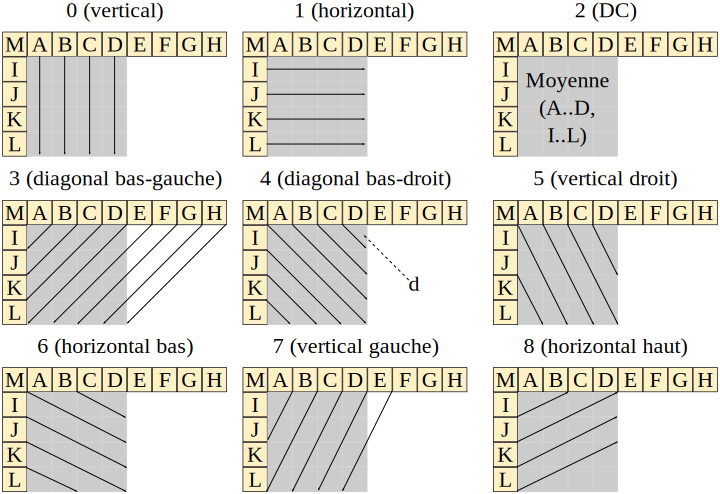
\includegraphics[width=\linewidth]{images/4x4PredictionModes.png}
\caption{Les modes prédictifs pour la luminance de blocs $4 \times 4$, inspiré
de~\cite{richardson2003}.}
\label{fig-4x4PredictionModes}
\LT{Refaire la \fig{fig-4x4PredictionModes} en $3 \times 3$}
\end{figure}

Nous pouvons, par exemple, définir la valeur de $\mathbf{d}$, le pixel situé
dans le coin supérieur droit du bloc $4 \times 4$ prédit par le mode~4
(diagonale sud-est). On obtient $\mathbf{d}$ à l'aide de la formule suivante~:
\SC{on ne voit pas 'd' sur la figure. Aussi on y parle de bas-droit et pas sud-est.}
\begin{equation}
\mathbf{d} = \text{round} \left(\frac{B + 2C + D}{4} \right)\:.
\end{equation}

La figure~\ref{fig-SAEPredictionBlocks} illustre la prédiction obtenue pour
chaque mode offert pour un bloc $4 \times 4$ ainsi que la somme de l'erreur
absolue (SAE) obtenue entre la prédiction et le bloc à encoder. Dans cet
exemple, le meilleur mode de prédiction serait 8, car il offre le plus petit
SAE, soit 203.

\begin{figure}[htb]
\fbox{\begin{varwidth}{\textwidth}\centering
\subfigure[Bloc~$4 \times 4$ à prédire.]{
\includegraphics[width=0.25\linewidth]{images/SAESource.png}
}\\
\subfigure[Résultats de prédiction \textit{intra} $4 \times 4$.]{
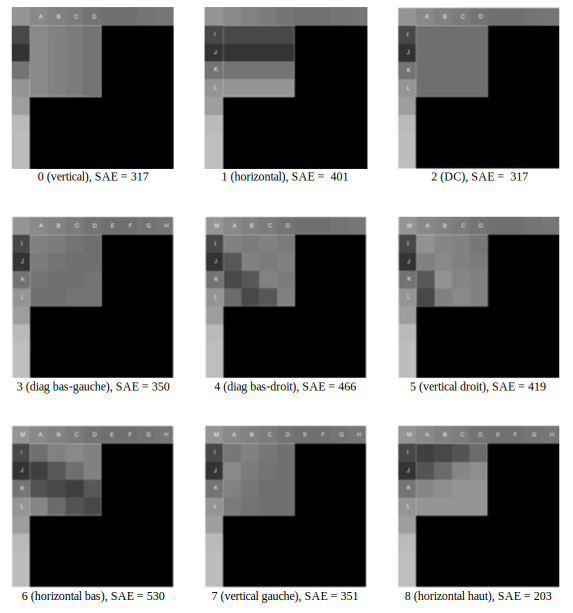
\includegraphics[width=0.85\linewidth]{images/4x4PredictionBlocks.png}
}
\end{varwidth}}
\caption{Comparaison des SAE issues des neuf modes de prédiction
\textit{intra} $4 \times 4$. Inspiré de~\cite{richardson2003}.}
\label{fig-SAEPredictionBlocks}
\end{figure}

En ce qui à trait à la prédiction des macroblocs $16\times16$, la norme H.264,
en prévoit quatre modes~: horizontal, vertical, DC et plane, tel qu'illustré à
la figure~\ref{fig-16x16PredictionModes}. Le mode DC utilise la moyenne des
pixels limitrophes horizontaux et verticaux, tandis que les trois autres
approches sont des extrapolations. Contrairement aux $4 \times 4$, les modes de
prédictions~$16 \times 16$ sont destinés aux surfaces lisses avec peu de
variation d'énergie. Ceci explique pourquoi le nombre de modes est restreint et
que ceux-ci sont plus simples.

\begin{figure}%[htb]
\centering
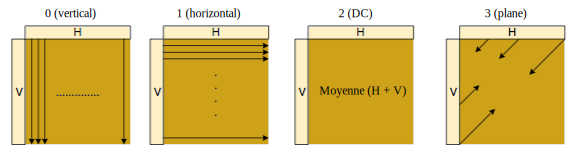
\includegraphics[width=\linewidth]{images/16x16PredictionModes.png}
\caption{Modes de prédiction de la luminance de blocs $16 \times 16$, inspiré
de~\cite{richardson2003}.}
\label{fig-16x16PredictionModes}
\end{figure}

En ce qui concerne les composantes chromatiques, elles se regroupent dans un
bloc $8~\times~8$, vu le sous-échantillonnage chromatique. Les mêmes types de
prédictions que pour les blocs $16~\times~16$ sont employés soient~: DC,
horizontal, vertical et plane. Ceci est dû au fait que dans les images
naturelles, les composantes chromatiques varient beaucoup moins que la
luminance~\citep{Wang2001}, ce qui en facilite la prédiction.
\end{subsection}
\end{section}


\begin{section}{La transformée}
\newcommand{\ltH}{\mathbf{H}}
Les approches présentées jusqu'à présent cherchent à éliminer la redondance
spatiotemporelle d'une séquence vidéo par l'utilisation de prédictions. Ces
prédictions reposent sur les corrélations intrinsèques aux données d'une
séquence vidéo. Ces prédictions sont imparfaites et requièrent que le
différentiel entre la prédiction et le bloc à encoder soit, lui aussi, encodé.
Toutefois, ce différentiel, appelé erreur résiduelle, possède une forte
autocorrélation. La transformée entière définie dans la norme H.264, a pour
objectif de décoreler spatialement l'erreur résiduelle afin d'en faciliter l'encodage. La
matrice de transformation suivante :
\begin{equation}
\ltH = \begin {bmatrix}
1 & 1 & 1 & 1\\
2 & 1 & -1 & -2\\
1 & -1 & -1 & 1\\
1 & -2 & 2 & -1
\end{bmatrix}
\end{equation}
possède des propriétés similaires à une transformée en cosinus discrète
(DCT) $4 \times 4$~\citep{malvar2003}, qui est très prisée pour son aptitude
à décorreler un ensemble de données.

La transformée entière possède plusieurs avantages par rapport à la DCT.
D'une part, elle est plus simple et requiert seulement des additions et
des décalages binaires (\textit{bit shift}). D'autre part, son résultat étant
entier implique qu'il n'y a pas de pertes fractionnaires (perte de précision) lors de la
transformée inverse.

H.264 applique sa transformée sur des blocs $4 \times 4$. Ceci la distingue de
ses prédécesseurs qui utilisent des blocs $8 \times 8$. L'utilisation de blocs
plus petits est justifiée par les améliorations substantielles de la  précision
des prédictions \textit{intra} et \textit{inter}, qui réduisent considérablement
le résiduel à transformer. De plus, l'utilisation de blocs plus petits réduit
grandement le bruit autour des bordures (souvent appellé \textit{ringing} ou
\textit{musquito noise}). L'ordre de balayage des différentiels de blocs $4
\times 4$ est présenté à la figure~\ref{fig-Transform}.

\begin{figure}[htb]
\centering
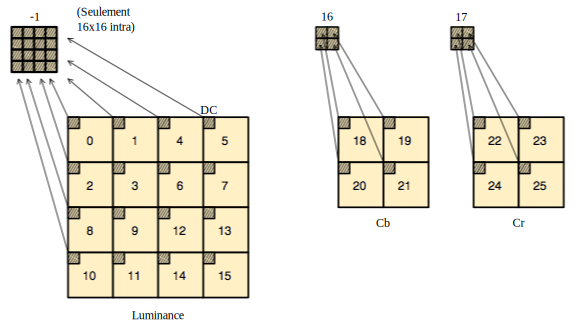
\includegraphics[width=\linewidth]{images/Transform.png}
\caption{Ordre de balayage des coefficients de blocs à
l'intérieur d'un macrobloc de l'erreur résiduelle lors de la transformée entière
$4 \times 4$. Inspiré de~\cite{richardson2003}.}
\label{fig-Transform}
\end{figure}

\end{section}

\begin{section}{La quantification}
Une nouveauté de la norme H.264 est qu'elle définit un paramètre de
quantification qui exerce un contrôle logarithmique sur le pas de quantification
alors que ses prédécesseurs utilisaient un contrôle linéaire. Le quantificateur
est scalaire et peut varier pour la luminance et les composantes chromatiques.
La valeur quantifiée $Z$ de la valeur transformée $W$ à la position $i,j$ est
défini comme étant :
\begin{equation}
Z_{ij} = \text{round}\left(\frac{W_{ij}}{Qstep}\right)
\end{equation}
où $Qstep$ est le pas de quantification et round la fonction d'arrondissement
afin d'obtenir des résultats entiers. La norme définit 52 valeurs de pas de
quantification indexées par le paramètre de quantification (QP). Une
augmentation de six de ce dernier double le pas de quantification. Ce grand
nombre de valeurs permet à l'encodeur une meilleure précision, en ce qui a trait
au compromis entre le débit binaire et à la qualité visuelle.
\end{section}

\begin{section}{L'encodage entropique}
La norme H.264 innove dans le domaine du codage entropique en séparant le codage
des paramètres de celui des données. Les paramètres sont représentés par des
codes numériques qui sont, eux mêmes, encodés avec des codes à longueur variable
appelés codes exponentiel-Golomb. Les valeurs des différentiels de prédiction
sont encodées soit avec un codage entropique à longueur variable (CAVLC) ou un
codage arithmétique binaire à contexte adaptatif (CABAC). Bien que CABAC offre
un gain de compression d'environ 10~\% par rapport à CAVLC, ce dernier est
prédominant dans les applications mobiles à cause de sa simplicité. C'est pour
cette raison que dans cet ouvrage, nous concentrons nos efforts exclusivement
sur le CAVLC.

Un encodage à longueur variable, comme celui présenté par \citep{huffman1952},
assigne des codes plus courts aux données plus fréquentes. Ceci implique que des
codes plus longs sont attribués aux autres données. Cependant, la faible
occurrence de longs codes assure que, comparé à un encodage à taille fixe,
l'encodage à taille variable requiert moins de bits pour encoder la séquence.

Dans un encodage à longueur variable, un bit erroné engendre une
désynchronisation beaucoup plus importante que pour un encodage à longueur
fixe. Le décodeur ne connaissant pas la longueur des codes, l'erreur se propage
jusqu'au prochain point de synchronisation prévue par la norme.
\end{section}

\begin{section}{Le filtre antiblocs}
Le filtre antiblocs, mieux connu sous son nom anglophone \textit{deblocking
filter}, a pour objectif de réduire l'apparence d'effets de bloc (variation
importante de la valeur des pixels en bordure de blocs). L'effet de bloc est
l'effet secondaire le plus important produit par les algorithmes de compression
vidéo présents dans la norme H.264. Il est le produit d'une discontinuité
spatiale provenant de variations d'encodage de blocs adjacents.

\begin{figure}[htb]

\centering
\subfigure[Sans filtre antiblocs]{
\includegraphics[width=0.47\linewidth]{images/ForemanWithoutDeblocking.png}
}
\subfigure[Avec filtre antiblocs]{
\includegraphics[width=0.47\linewidth]{images/ForemanWithDeblocking.png}
}
\caption{Performance du filtre antiblocs pour une trame fortement
compressée~\citep{schafer2003}.}
\label{fig-Deblocking}
\end{figure}

Le filtre antiblocs agit en bordure de blocs dans le but de lisser les
variations importantes d'intensités des valeurs de pixels, La
\fig{fig-Deblocking} démontre l'efficacité du filtre antiblocs appliqué sur une
trame fortement compressée. Beaucoup plus qu'un simple filtre, le filtre
antiblocs tient compte du pas de quantification ainsi que du type de prédiction
utilisé pour encoder les blocs, afin d'ajuster l'intensité du lissage.

La norme H.264 définit deux seuils qui régissent le comportement du filtre
antiblocs. Soit $\alpha$ pour l'écart entre les pixels en bordure de deux
blocs~:
\begin{equation}
\left| p_0 - q_0 \right| < \alpha(\text{Indice}_A)
\end{equation}
et $\beta$ pour l'écart entre les pixels à la bordure d'un même bloc~:
\begin{align}
\left| p_1 - p_0 \right| < \beta(\text{Indice}_B)\\
\left| q_1 - q_0 \right| < \beta(\text{Indice}_B)
\end{align}
\begin{figure}[htb]
\centering
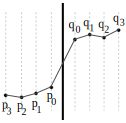
\includegraphics[scale=0.65]{images/BlockyEdge.png}
\caption{Visualisation unidimensionnelle d'une bordure de bloc qui requiert
l'intervention du filtre antiblocs. Inspiré de~\citep{list2003}.}
\label{fig-BlockyEdge}
\end{figure}
où $p_i$ et $q_i$ sont les pixels en bordure de blocs tel qu'illustré à la
figure~\ref{fig-BlockyEdge}. L'encodeur peut biaiser les indices à l'aide
d'un décalage tel que
\begin{align}
\label{eq-IndicesA}
\text{Indices}_A &= \min(\max(0,\text{QP}+\text{Decalage}_A), 51)\\
\label{eq-IndicesB}
\text{Indices}_B &= \min(\max(0,\text{QP}+\text{Decalage}_B), 51)\:.
\end{align}
La plage de valeur de 0 à 51 représente les valeurs possibles du paramètre de
quantification (QP). Cela dit, aux formules~\ref{eq-IndicesA} et
\ref{eq-IndicesB}, QP est le paramètre de quantification moyen entre les deux
blocs évalués. Les valeurs des seuils $\alpha$ et $\beta$ sont définies à l'aide
des formules suivantes~:
\begin{align}
\alpha(x) &= 0.8(2^{x/6}-1)\\
\beta(x) &= 0.5x-7
\end{align}

Afin de savoir si un lissage doit être appliqué et, si oui, à quelle
intensité, le paramètre d'intensité de la bordure (bS) est défini selon des
règles basées sur le mode d'encodage. Celles-ci sont résumées dans la table
\ref{tab-FilteringRules}.

\begin{table}[htb]
\caption{Règles guidant l'intensité du filtre antiblocs en fonction des
conditions d'encodages.}
\label{tab-FilteringRules}
\vspace{1em}
\centering
\begin{tabular}{ l l }
\hline
Condition d'encodage & Intensité \\
\hline
Prédiction Intra et en bordure de macrobloc & 4 (Lissage fort)\\
Prédiction Intra & 3 \\
Prédiction Inter et présence de résiduel & 2 \\
Différence des vecteurs de mouvement $\geqslant$ 1 & 1 \\
Prédiction Inter avec des trames de références différentes& 1 \\
Sinon & 0 (Aucun lissage) \\
\hline
\end{tabular}
\end{table}

Comme le démontre la table~\ref{tab-FilteringRules}, le type de
prédiction et les conditions d'encodage produisent différents degrés d'effet
de bloc. C'est pourquoi, il est crucial que le filtre soit ajustable. De plus,
les seuils $\alpha$ et $\beta$ permettent de prendre en compte la texture propre
à l'image afin de ne pas lisser des variations de valeurs de pixels propres à
l'image situés en bordure de blocs.

L'usage du filtre antiblocs permet, pour un même niveau de qualité visuelle
(mesuré avec le PSNR), d'obtenir une réduction du débit de 5 à 10~\% selon le
contexte~\citep{list2003}. L'ajout, à la norme H.264, du caractère obligatoire
de ce mécanisme différencie cette dernière de ses prédécesseurs. Quoique
plusieurs utilisent des filtres antiblocs, peu les rendent obligatoires. Son
ajout dans la chaîne d'encodage décodage fait en sorte que ses améliorations
sont prises en compte lors des prédictions inter-image.
\end{section}

\SC{petite conclusion et les points importants à retenir dans ce chapitre? par exemple, qu'une erreur d'un bits peut avoir de grandes conséquences sur le décodage}

\bibliographystyle{bibETS}
\bibliography{h264}

\end{chapter}

\end{document}
